\documentclass{article}
\usepackage{graphicx}
\graphicspath{ {./immagini/}}
\usepackage{blindtext}
\title{Funzioni}
\begin{document}
\section{Proprieta funzioni}
Le funzioni sono una corrisposndenza degli elementi di Insieme A ad un elemento di B\\
\\
$F: A \to B \quad \quad A,B \subseteq R$\\

$x \in A \quad \to \quad f(x) \in B \quad \to \quad $ dobbiamo descrivere il grafico\\

$\{ (x,F(x): x \in A \} \subseteq R x R$ (prodotto cartesiano)\\
\\
\\
Notazioni e definizioni:\\
- Funzione iniettiva: $\forall x_{1},x_{2} \in A \quad F(x_{1})=F(x_{2}) \to x_{1}=x_{2}$\\
- Funzione surriettva su B: $\forall y \in B \quad \exists x \in A :F(x)=y$\\
- Funzione biunivoca se e' sia suriettiva che inniettiva: $\forall y \in B !\exists x \in A:F(x)=y$\\
\\
se la funzione e' biunivoca invertendo la corrispondenza ho la funzione inversa $\to F^{-1}(y)=x$ (ribaltando il grafico di 90 gradi verso destra)\\
\\
Es. $F(x)=x^{2} \quad D=R, A \subseteq, B \subseteq R$ (D=dominio e serve a trovare un senso alla funzione)$A=R, B=R$\\
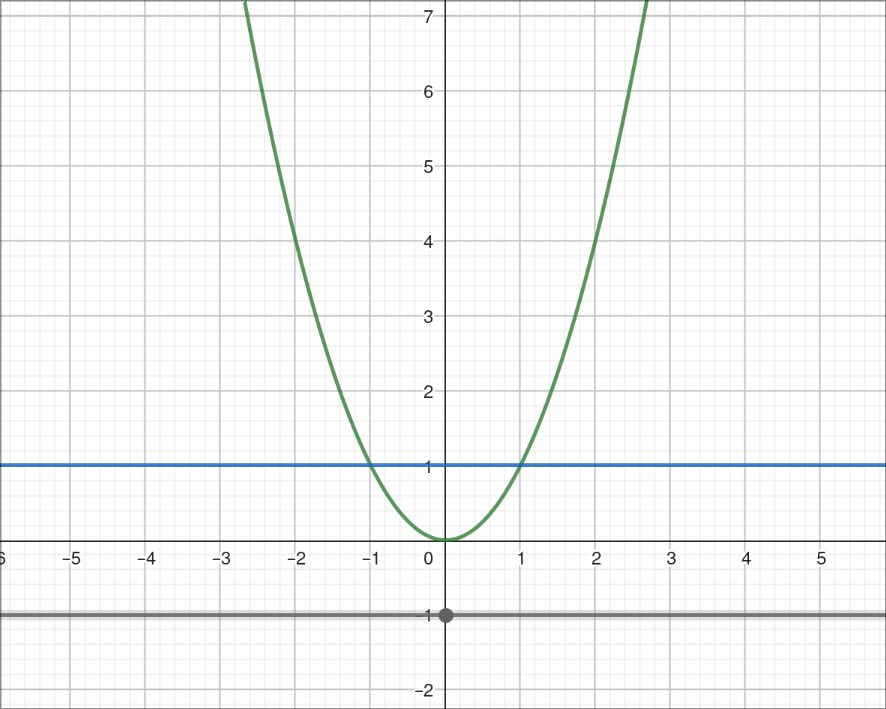
\includegraphics{1-Lezione-2-esempio.png}
\\
\\
\\
F non e inniettiva\\
$F(1)=F(-1)=1$\\
\\
F non e surriettiva\\
$F(x)=-1$ non ha soluzione per $x \in A$\\
\\
\\
Se mettiamo come dominio: $A=R \quad e \quad B=[0,+ \infty) =R+ \to$ non e inniettiva ma surriettiva perche con il nuovo domininio non prendiamo numeri negativi\\
\\
\\
\\
\\
- $A=[0,+ \infty)$\\
- $B=[0,+ \infty)$\\
\\
con questo dominio la funzione diventa biunivoca\\
\\
$F^{-1}(x)=\sqrt x$
\\
\\
\section{Funzioni Elementari}

\textbf{-Funzione retta}\\
$\to F(x)=mx + q$\\
q= intersezione nell asse delle y\\
m= pendenza della retta\\
\\
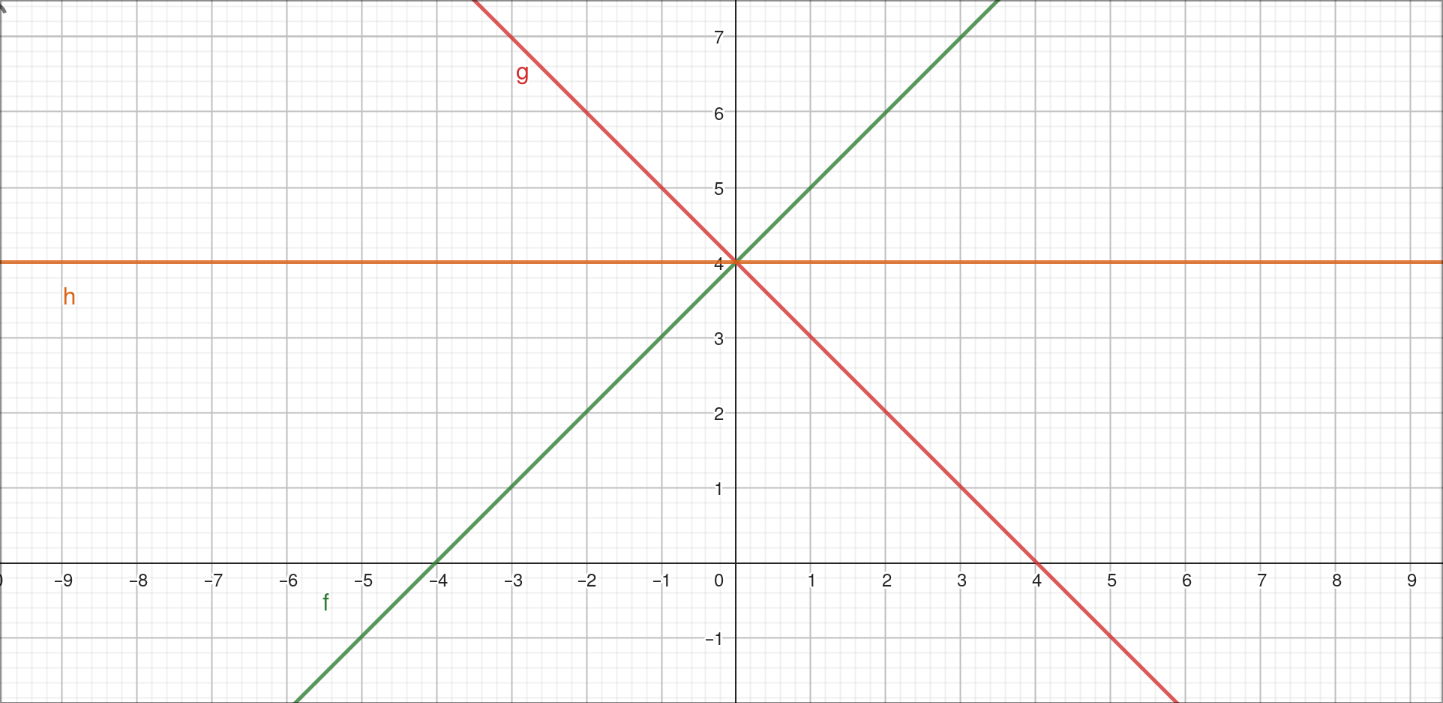
\includegraphics{./immagini/funzione-retta.png}
\\
F e' crescente in\\
$A \subseteq D$ se $\forall x_{1},x_{2} \in A \quad x_{1} \leq x_{2} \to F(x_{1}) \leq F(x_{2})$
\\
F e' decrescente in\\
$A \subseteq D$ se $\forall x_{1},x_{2} \in A \quad x_{1} \leq x_{2} \to F(x_{1}) \geq F(x_{2})$\\
\\
\textbf{-Funzione valore assoluto}\\
D=R\\
$F(x)=|x|=\{ x \quad se \quad x \geq 0,\{ -x \quad se \quad x \leq 0\}$\\
\\
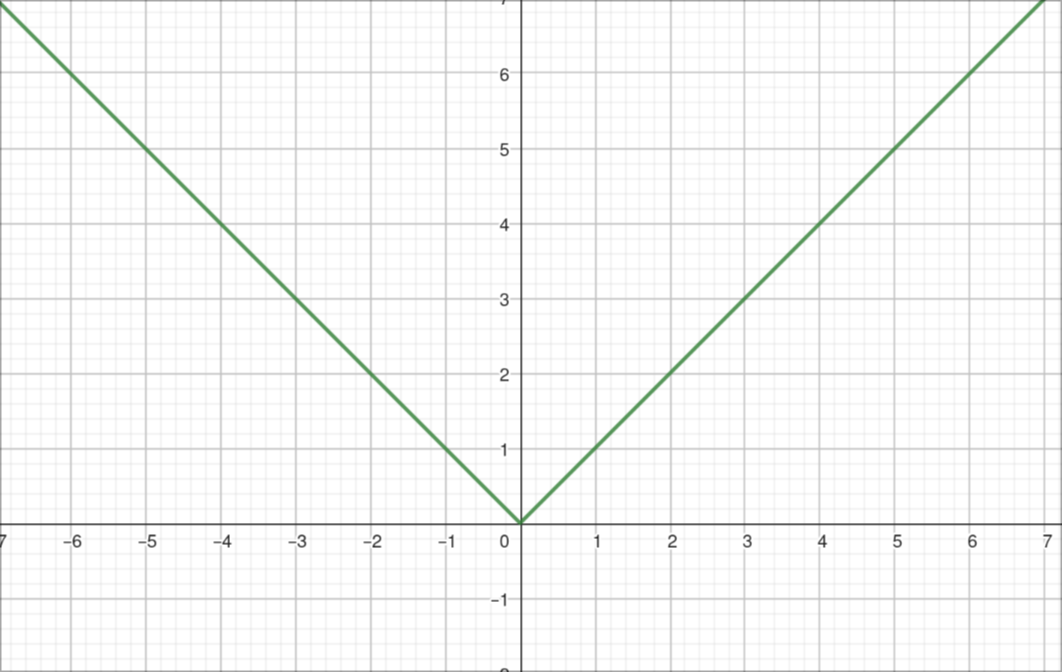
\includegraphics{./immagini/funzione-modulo.png}
\\
\textbf{-Funzione potenza}
\\
$F(x)=x^n \quad n \in Z , \quad n \neq 0$
$n>0$ pari=simmetria per l asse delle x\\
\\
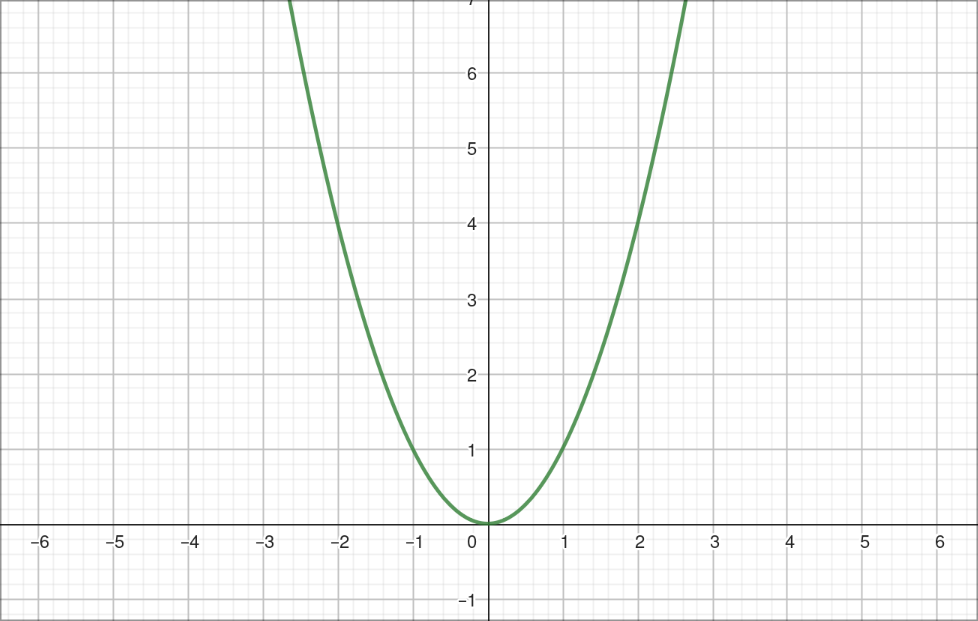
\includegraphics{./immagini/funzione-potenza-pari.png}
\\
\\
$n>0$ dispari=simmetria per l origine\\
\\
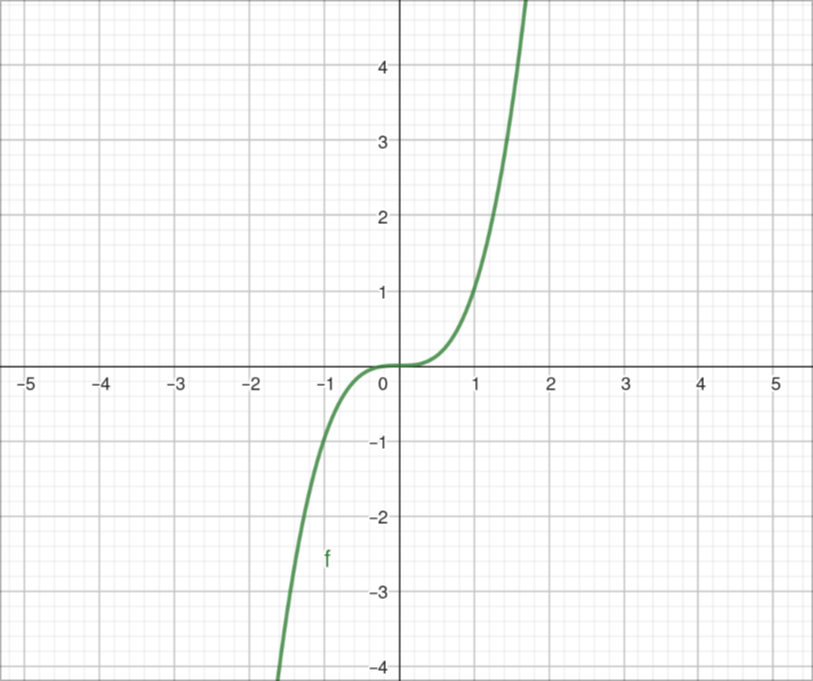
\includegraphics{./immagini/funzione-potenza-dispari.png}
\\
\\
F si dice pari in D se $\forall x \in D, -x \in D\quad e \quad F(x)=F(-x)$\\
F si dice dispari in D se $\forall x \in D, -x \in D\quad e \quad F(x)=-F(-x)$\\
\\
$n<0 $ pari\\
\\
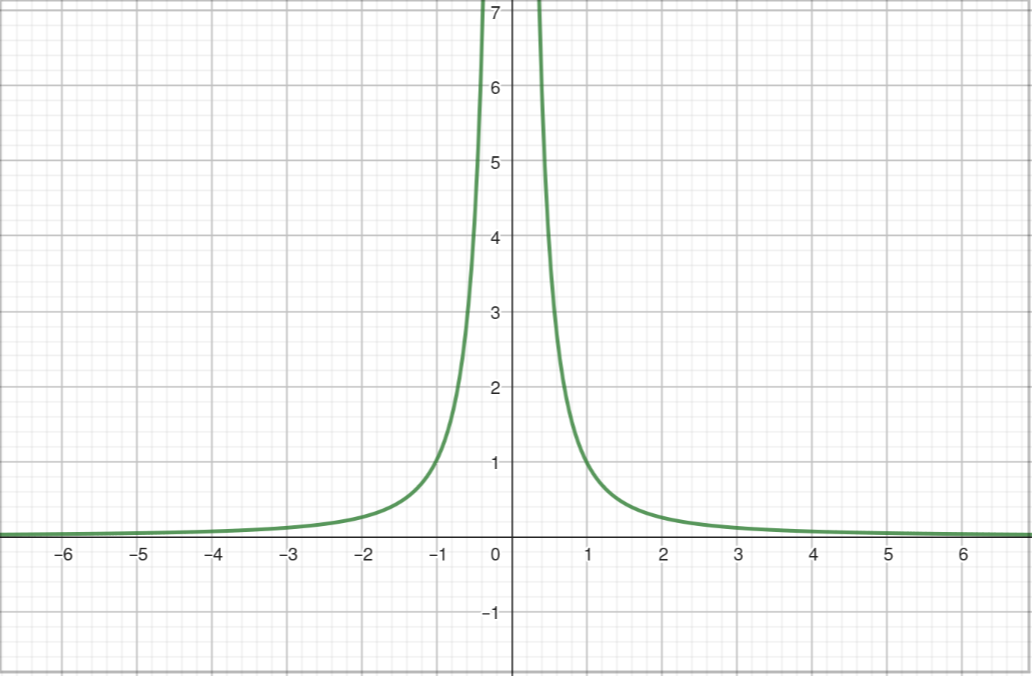
\includegraphics{./immagini/funzione-potenza-pari-minore.png}
\\
\\$n<0 $ dispari\\
\\
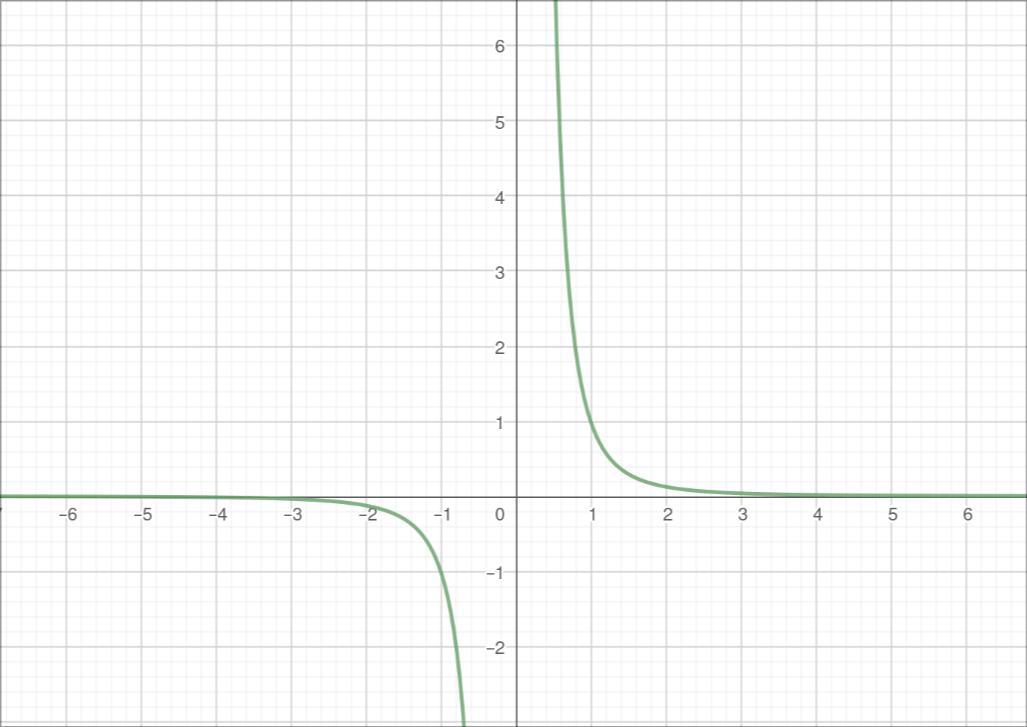
\includegraphics{./immagini/funzione-potenza-dispari-minore.png}
\\
\textbf{-Funzione radice n-esima} $n \in N^{+}$\\
se n e' pari\\
\\
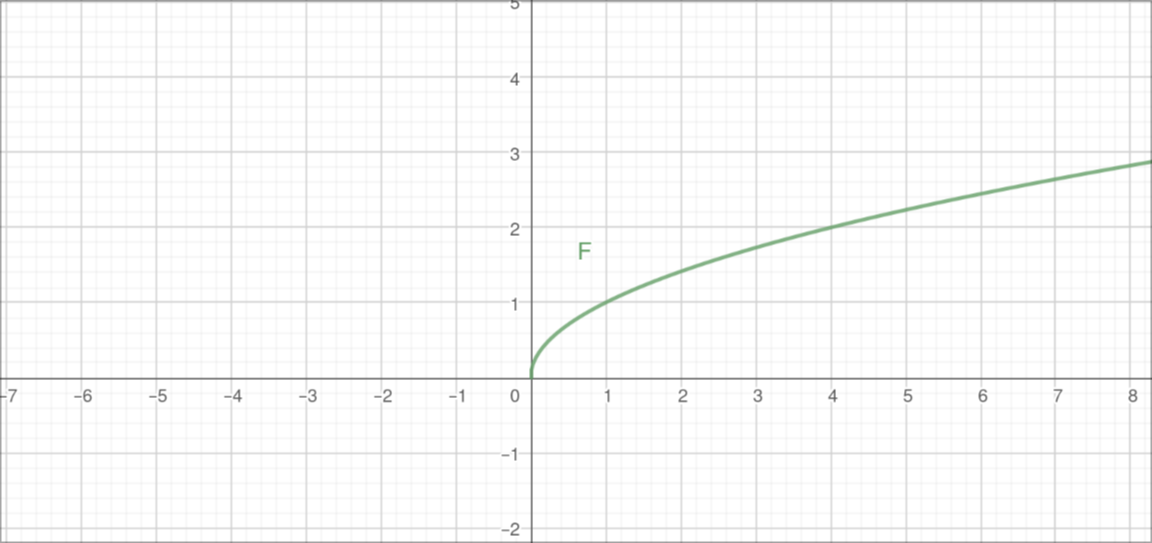
\includegraphics{./immagini/funzione-radice-pari.png}
\\
\\
se n e' dispari\\
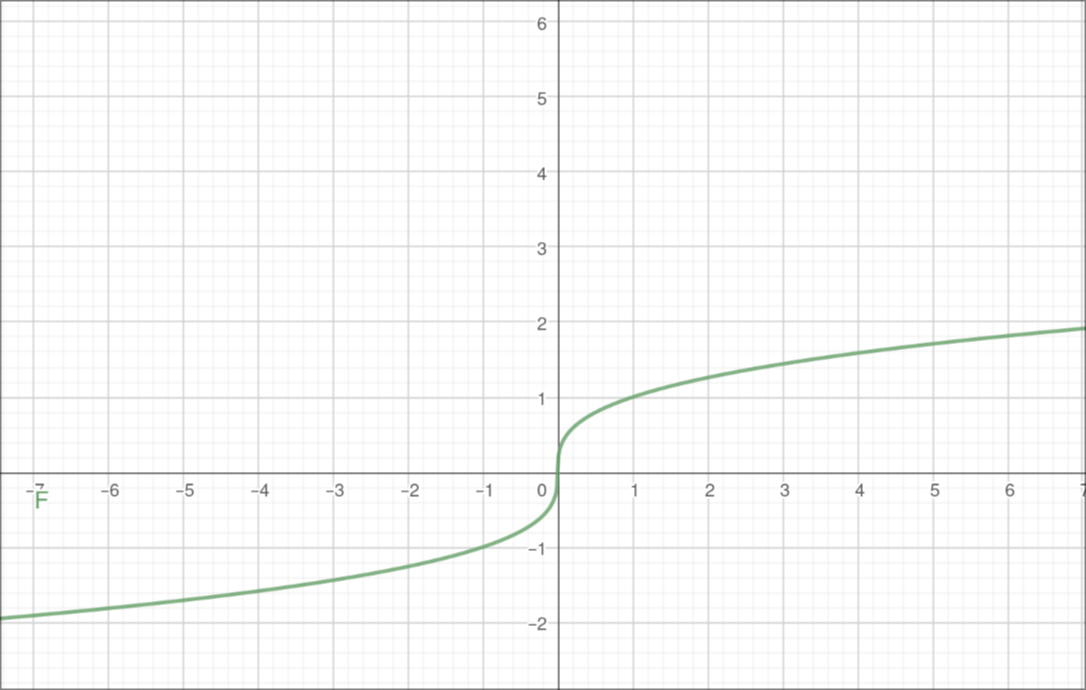
\includegraphics{./immagini/funzione-radice-dispari.png}
\\
\textbf{-Funzione esponenziale}\\
$F(x)=a^{x} \quad a > 0 \quad x \ne 1, \quad (a = e)$\\
\\
\\
$a>1$
\\
\\
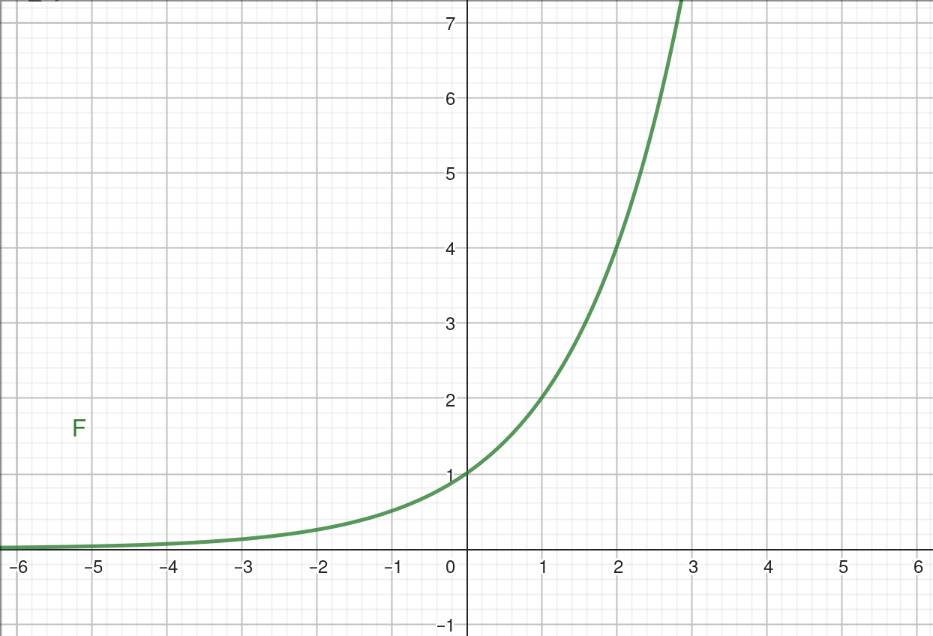
\includegraphics{./immagini/funzione-esponenziale.png}
\\
\\
$0<a<1$
\\
\\
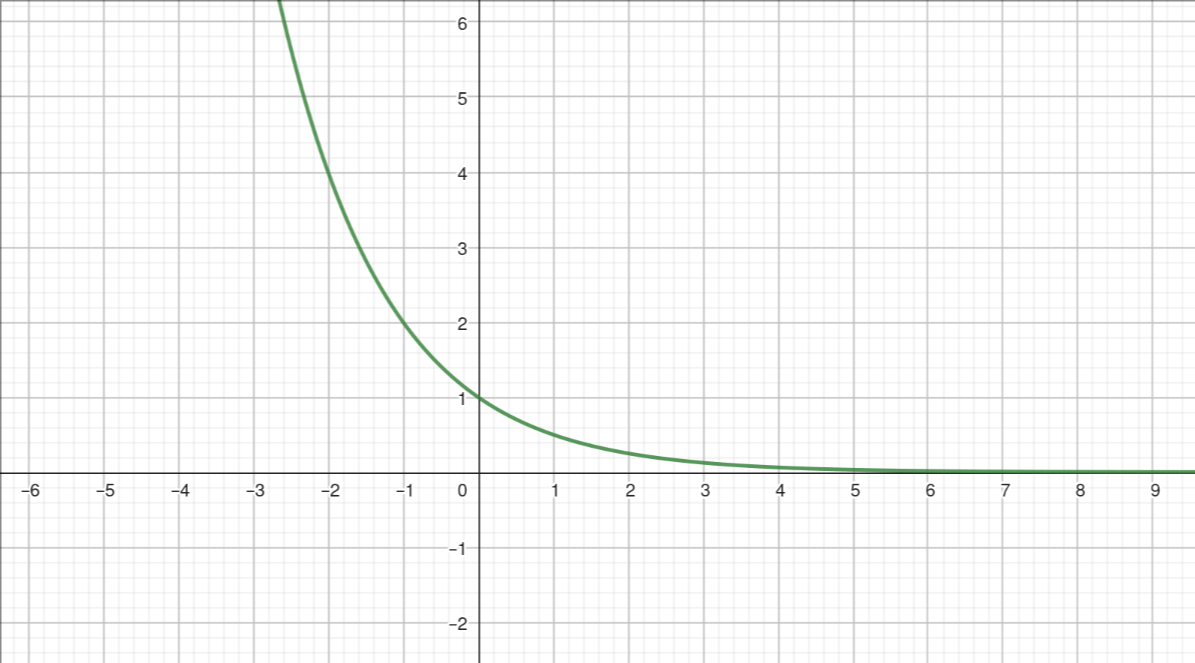
\includegraphics{./immagini/funzione-esponenziale-negativa.png}
\\
\\
\textbf{-Funzione logaritmiche} (inversione di quella esponenziale)\\
$F(x)=log_{a}(x)$\\
D=$(o,+\infty)$\\
\\
\\
$a>1$\\
\\
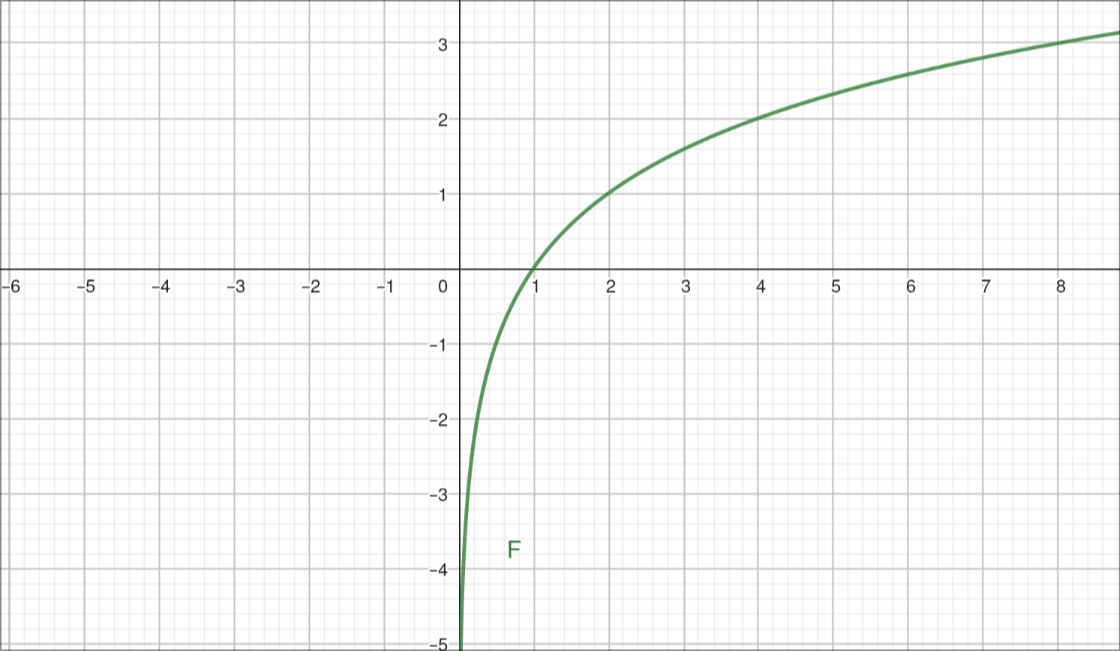
\includegraphics{./immagini/funzione-logaritmica.png}
\\
\\
$0<a<1$\\
\\
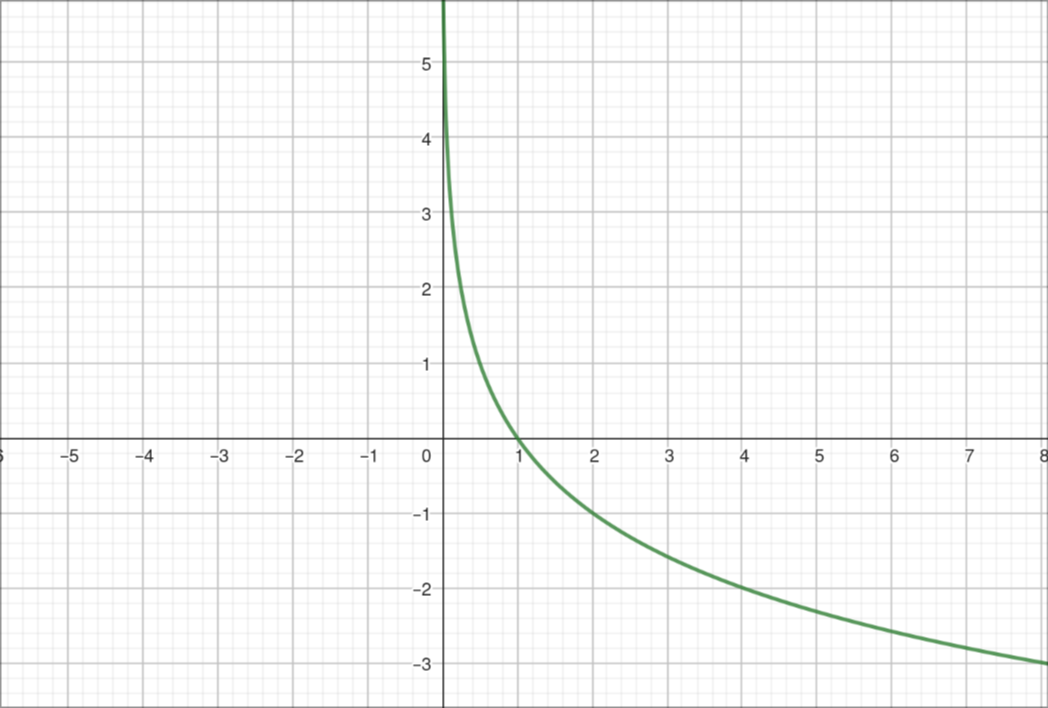
\includegraphics{./immagini/funzione-logartmica-negativa.png}
\\
\\
\textbf{-Proprieta logaritmiche}\\
$log(x^{\alpha})=\alpha log(x)$\\
$log(x_{1}) + log(x_{2})=log(x_{1} \star x_{2})$\\
$\forall x \in R \quad log_{\alpha}(\alpha^{x})=x \quad a^{log_{a}(x)}=x \quad \forall x>0$\\
\\
\\
\textbf{-Funzioni logaritmiche}\\
$F(x)=sin(x) \quad D=R \quad T=2 \pi$ e' dispari\\
\\
(grafico)
\\
\\
$F(x)=cos(x) \quad D=R \quad T=2 \pi$ e' dispari\\
\\
(grafico)\\
\\
$F(x)=arcsin(x) \quad D=[-1,1] \quad T=2 \pi$\\
\\
(grafico)
\\
\\
$F(x)=arccos(x) \quad D=[1,-1] \quad T=2 \pi$\\
\\
(grafico)
\\
\\
$F(x)=tan(x) \quad D= R/\{\frac{\pi}{2}+k \pi \} \quad T=2 \pi$\\
$tan(x)=\frac{sin(x)}{cos(x)}$\\
\\
(grafico)
\\
\\
$F(x)=arctan(x)$\\
\\
(grafico)
\\
\\
\textbf{-Operazioni sui grafici}\\
\\
$-F(x)+-a \to$ slitta il grafico sull asse delle y\\
$-F(x+-a) \to$ slitta il grafico sull asse delle x (f(x-a) slitta il grafico verso destra)\\
$-F(x)$ capovolge verso la x\\
$-F(-x)$ specchia verso la y\\
$-F(|x|)$ specchia il contenuto  per l asse delle y della parte di funzione che si trova nel primo quadrante\\
$-F(- |x|)$ e' l inverso di quella sopra\\
$- |F(-x)|$ prende la parte sotto all asse della x e la ribalta sopra\\

\end{document}
